% THIS IS SIGPROC-SP.TEX - VERSION 3.1
% WORKS WITH V3.2SP OF ACM_PROC_ARTICLE-SP.CLS
% APRIL 2009
%
% It is an example file showing how to use the 'acm_proc_article-sp.cls' V3.2SP
% LaTeX2e document class file for Conference Proceedings submissions.
% ----------------------------------------------------------------------------------------------------------------
% This .tex file (and associated .cls V3.2SP) *DOES NOT* produce:
%       1) The Permission Statement
%       2) The Conference (location) Info information
%       3) The Copyright Line with ACM data
%       4) Page numbering
% ---------------------------------------------------------------------------------------------------------------
% It is an example which *does* use the .bib file (from which the .bbl file
% is produced).
% REMEMBER HOWEVER: After having produced the .bbl file,
% and prior to final submission,
% you need to 'insert'  your .bbl file into your source .tex file so as to provide
% ONE 'self-contained' source file.
%
% Questions regarding SIGS should be sent to
% Adrienne Griscti ---> griscti@acm.org
%
% Questions/suggestions regarding the guidelines, .tex and .cls files, etc. to
% Gerald Murray ---> murray@hq.acm.org
%
% For tracking purposes - this is V3.1SP - APRIL 2009

\documentclass{acm_proc_article-sp}
\usepackage{url}
\begin{document}

\title{QueryMed: For Querying Biomedical Data on the Web\titlenote{Interested readers are advised to visit http://code.google.com/p/querymed to learn more about QueryMed.}}


\numberofauthors{2}
\author{
\alignauthor Oshani Seneviratne\\
       \affaddr{Massachusetts Institute of Technology}\\
       \affaddr{Cambridge, MA}\\
       \affaddr{USA}\\
       \email{oshani@csail.mit.edu}
\alignauthor Rachel Sealfon\\
       \affaddr{Massachusetts Institute of Technology}\\
       \affaddr{Cambridge, MA}\\
       \affaddr{USA}\\
       \email{rsealfon@csail.mit.edu}
}


\maketitle
\begin{abstract}

QueryMed is a query builder and result set visualizer for biomedical data, that allows end-users to easily construct and run translational medicine queries across multiple data sources. It allows users to select the data sources they wish to use, drawing on their specialized domain knowledge to decide the most appropriate data sources to query.  User input is translated into SPARQL~\cite{SPARQL} queries and executed at the relevant endpoints. The results are presented in an intuitive user interface that allows query refinement and filtering.  

\end{abstract}

%\category{H.4}{Information Systems Applications}{Miscellaneous}
\keywords{Biomedical Ontologies, SPARQL, Query Federation, Query Building, Semantic Web, User Interfaces} 

\section{Introduction}

Answering many medically and biologically relevant questions with information available on the Web requires searching, filtering, and combining information from multiple data sources.  For example, a physician who knows a patient's symptoms, current medications, and genotype may wish to determine the treatment plan and identify clinical trials for which the patient is eligible for.  However, there is no single data source that the physician can use to figure out the answers. The information that the physician needs must be gathered from numerous data sources such as Pubmed, DailyMed, Drugbank, LinkedCT, Diseasome,  and Gene Ontology \cite{Pubmed, DailyMed, Drugbank, LinkedCT, Diseasome, GO}. The quantity of publicly available data in the biomedical domain has dramatically increased over the recent years. With the linked open data movement, the Semantic Web community has been very proactive in converting these rich information resources to RDF~\cite{LinkingData}.  The biomedical domain is in fact among the early successes of the Semantic Web, due to the rapidity with which the community has made its data available in RDF triple stores~\cite{Yip}.  However, to exploit the abundance of this data on the Web, there is a need for easy-to-use systems that do not require the end-user to have knowledge of the underlying  structure of the data or the ontologies used in describing the data. These systems should also support the queries to be run across multiple data sources.  There is also a  need for efficient hybrid interfaces that allow both browsing and querying of data~\cite{Jentzsch}.  

%Her question must be broken up into discrete pieces that can be executed individually at one data source at a time.  Since the physician must search many data sources in order to find an answer to her single question, she requires a system that can automatically run queries over multiple data sources. Also, the physician may not know SPARQL syntax, the location of the SPARQL endpoints (i.e. data sources), or the structure of the ontologies used to describe the data in the endpoints. She is likely to want an intuitive way to query and to display the query results.  Developing intuitive ways to query multiple SPARQL endpoints and to display results is both an important and a challenging problem.  Our system, QueryMed, allows users with no knowledge of the SPARQL query language or the structure of the underlying ontologies to easily run queries across multiple SPARQL endpoints.


\section{Overview}

QueryMed allows querying of multiple biomedical data sources very easily.  Queries can be run against a default list of SPARQL endpoints, or against a set of user-defined endpoints. The system automatically translates the user input into a SPARQL query for each individual endpoint, executes the query, combines the results, and returns them to the user.  If the user is not happy with the results, the query can be refined  by iteratively modifying the original terms used in the query, and by filtering the result set.  The advanced query functionality of QueryMed enable the user to easily construct complex logical SPARQL queries that take advantage of the underlying structure of the data. The simple user interface of QueryMed is designed to be intuitive for users with no knowledge of SPARQL. A general overview of QueryMed architecture is shown in Figure \ref{fig:arch_details}.

\begin{figure}
\centering
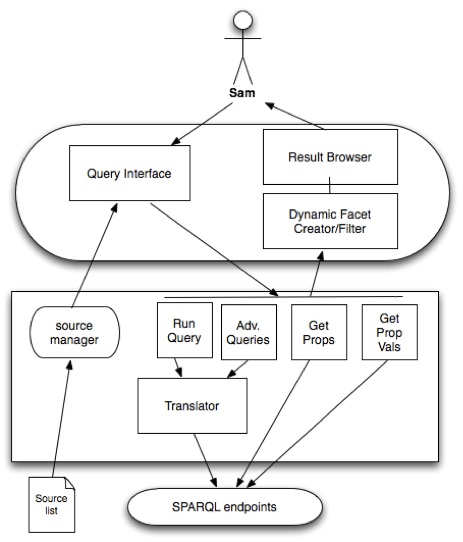
\epsfig{file=images/architecture_detail.jpg, width=3in}
\caption{QueryMed Architecture}
\label{fig:arch_details}
\end{figure}

\subsection{QueryMed in Action}

Imagine a scenario in which a physician called Sam, is interested in finding freely available resources related to coronary artery disease.  Using QueryMed Sam first tries a basic search over all default resources, by entering ``coronary artery disease" in the search box. Sam then sees a list of disease names in the Diseasome database and drugs in DailyMed and Drugbank that relate to coronary artery disease displayed in a table.  He can then filter the results using additional search terms.  For example, he knows that the route of administration of the drug that he is looking for is injection, so he filters the drug query results on the route of administration field using the query term ``injection."  he then prints the table of results. he is now interested in finding relevant clinical trials for her patient.  However, the clinical trial database (LinkedCT~\cite{LinkedCT}) is not in the default set of endpoints, so he selects the ``Refine Query" option to choose additional endpoints to search.  he sees a list of default endpoints, and selects the ``Add" option to include an additional endpoint.  After entering the name and URL of the LinkedCT endpoint, he is able to search for clinical trials for which her patient may be eligible.  He is also interested in further refining her search, so he uses the advanced search option to construct a query that takes advantage of the underlying structure of the RDF data in the database.  He searches the data available in the Diseasome endpoint for a list of diseases whose class is ``Cardiovascular" or for which the associated gene is ``ABCA1."  Using the QueryMed advanced search interface, the complex SPARQL query corresponding to his question is automatically constructed, and he can view the query results conveniently displayed in a table. A demo describing this scenario is available at \url{http://dig.csail.mit.edu/2010/Papers/www-ws-colab-science/videos/querymed-demo.mov}.

\section{Related Work}
\label{related}

A number of existing tools aim to provide a user-friendly interface for browsing Semantic Web data, or to allow users to perform federated queries. The SMART query tool~\cite{Battista} is a Web-based application designed to allow biologists to run queries written in Manchester OWL syntax. Unlike in SMART, QueryMed allows constructing queries intuitively by specifying keywords for user selected properties, to iteratively refine query results, and to dynamically add additional endpoints. GoWeb~\cite{Dietze} allows users to perform a hybrid search, running keyword-based queries and then filtering based on ontological concepts. However, GoWeb functions as a search engine that has in-built ontological background knowledge to improve the search results, whereas QueryMed utilizes user input in constructing SPARQL queries without any ontological backing.  BioGateway~\cite{Antezana} provides a Web interface to query a provided single SPARQL endpoint that includes graphs from several biomedical resources. However, BioGateway does not facilitate dynamic addition of endpoints like in QueryMed. Another, query builder, Twinkle~\cite{Dodds}, offers a stand-alone graphical user interface to load and edit SPARQL queries. Our system differs from the Twinkle, because in QueryMed, the user can provide input in the form of keywords, and has the option to restrict the query if she wishes to run a more precise query. Most SPARQL query engines are designed to run queries against individual endpoints. But it is often useful to draw on multiple web resources in answering a query. The DARQ  system \cite{Quilitz} is designed to allow the user to run integrated queries against multiple SPARQL endpoints. But it does not offer a graphical user interface as in QueryMed to facilitate use by biomedical domain experts who are not familiar with SPARQL query syntax.

\section{Conclusion}
\label{conclusion}

The main contributions of QueryMed are: dynamic construction of complex SPARQL queries based on intuitive user input; dynamic addition of user-specified endpoints; and ability to run queries over multiple endpoints. Because it is flexible and easy to use, we believe that it will be of immense value to the biomedical community.  We also believe that developing systems such as such as QueryMed, which make SPARQL endpoints  easily accessible to end-users, will entice more people to expose their data as linked open data thus promoting the growth of the LODD cloud.


\bibliographystyle{abbrv}
\bibliography{sigproc}  % sigproc.bib is the name of the Bibliography in this case
\end{document}
